\documentclass[12pt,a4paper]{article}
\setlength{\hoffset}{-0.8in} \setlength{\voffset}{-0.55in}
\setlength{\textheight}{240mm}
\setlength{\textwidth}{150mm}
\setlength{\headheight}{14pt}
% \usepackage{fancybox,latexsym,epic,eepic,epsfig}
\usepackage{amsmath,enumerate,ifthen}
\usepackage{amssymb}
\usepackage{framed}
\usepackage{times}
\usepackage{multicol}
\usepackage{fancyhdr}\usepackage{graphicx}
% \input def.tex

\usepackage{pgfpages}
% \pgfpagesuselayout{2 on 1}[a4paper, landscape]

\newcommand{\R}{\mathbb{R}}
\newcommand{\N}{\mathbb{N}}
\newcommand{\bs}{\bigskip}


\begin{document}
	\section*{Question 4}
	4) Vectors / Systems of Linear Equations
	




	
	\subsection*{Part A. Cross Product abd Scalar Triple Product}
 Calculate the scalar triple product
	
	\[u\cdot (v\times w)\]
	
	for
	
	\begin{enumerate}
		\item $u=(1,3,5)$; $v=(0,5,3)$; $w=(3,0,7)$;
		
		\item $u=(0,1,2)$; $v=(5,0,1)$; $w=(2,2,2).$
	\end{enumerate}


 
 \vspace{0.25cm}Calculate the cross products $u\times
 u^{\prime}$, $v\times v^{\prime}$, $w\times w^{\prime}$, where
 $u$, $u^{\prime}$, $v$, $v^{\prime}$, $w$, $w^{\prime}$ are given
 in  Question $6$.
 	
\subsection*{Part A. Triangle Inequality}
%==============================================%

Cauchy Schwarz Identity

Triangle Identity


\begin{enumerate}
	\item For the vectors given below, evaluate the following expressions where it is possible.
	\begin{equation*}
	\vec{u}=\left[ \begin{array}{c} 1 \\ 2 \\ 3 \end{array}\right],
	\vec{v}=\left[ \begin{array}{c} -1 \\ 0 \\ 4 \end{array}\right],
	\vec{x}=\left[ \begin{array}{c} 3 \\ 4 \end{array}\right],
	\vec{y}=\left[ \begin{array}{c} -4 \\ 3 \end{array}\right],
	\vec{w}=\left[ \begin{array}{c} 1 \\ 0\\ 2 \\ -5 \end{array}\right],
	\vec{z}=\left[ \begin{array}{c} 2 \\ 2 \\ 2 \\ 3 \end{array}\right]
	\end{equation*}
	\begin{multicols}{3}
		\begin{enumerate}
			\item $2\vec{u} + 3\vec{v}$
			\item $3\vec{u} - \vec{v}$
			\item $\vec{x} + 3\vec{v}$
			\item $2\vec{z} - \vec{w}$
			\item $\vec{u}+\vec{x}$
			\item $\vec{v}+\vec{w}$
			\item $\vec{u}\cdot \vec{v}$
			\item $\left(2\vec{u}\right)\cdot \left(3\vec{v}\right)$
			\item $\vec{x}\cdot \vec{y}$
			\item $\vec{w} \cdot \vec{z}$
			\item $\vec{w} \cdot (\vec{z}+\vec{w})$
			\item $|\vec{x}|$
			\item $|\vec{w}|$
			\item $|\vec{y}|+|\vec{w}|$
		\end{enumerate}
	\end{multicols}
	
	\item
	Calculate the angles between the pairs $\vec{u},\vec{v}$, $\vec{x},\vec{y}$, and $\vec{w},\vec{z}$ from the previous question. Give your answers in both radians and degrees.
	
	\item
	Calculate the area of the parallelogram spanned by the vectors $\vec{x}$ and $\vec{y}$.
	\item
	Show that the volume of the parallelopiped spanned by the vectors $\vec{u},\vec{v}$ and $2\vec{u}+3\vec{v}$ is zero.
	
	\item
	
\end{enumerate}

\begin{enumerate}
	\item
	For each of the following systems of linear equations, write down the corressponding coefficient matrix $A$, vector of unknowns $\vec{x}$, and vector of right hand sides $\vec{b}$ so that the system can be expressed in the form $A\vec{x}=\vec{b}$
	\begin{multicols}{3}
		\begin{enumerate}
			\item
			\begin{align*}
			2x+3y&=1\\
			5x+7y&=3
			\end{align*}
			\item\begin{align*}
			2x+3y+4z&=1\\
			x-2y+2z&=7\\
			3x+2y+z&=0.2
			\end{align*}
			\item
			\begin{align*}
			3x+y+z&=1\\
			y+4z&=-4\\
			x-y&=2
			\end{align*}
		\end{enumerate}
	\end{multicols}
	\item
\end{enumerate}
%\begin{wrapfigure}{r}{0.5\textwidth}
%    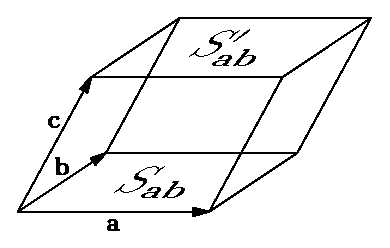
\includegraphics[width=0.5\textwidth]{par3_tut}
%    \vspace{-5em}
%\end{wrapfigure}

Let the vectors $\vec{a},\vec{b},\vec{c}$ be given by
\begin{equation*}
\vec{a}=\left[ \begin{array}{c} 2 \\ 0 \\ 0 \end{array}\right],
\vec{b}=\left[ \begin{array}{c} 2 \\ 1 \\ 0 \end{array}\right],
\vec{c}=\left[ \begin{array}{c} 2 \\ 0 \\ 1 \end{array}\right]
\end{equation*}
These vectors span a three dimensional parallelopiped as shown in the figure to the right.

\begin{enumerate}
	\renewcommand{\theenumi}{\roman{enumi})}
	\renewcommand{\labelenumi}{\theenumi}
	{\setlength\itemindent{3em} \item
		Find the area of the parallelogram $S_{\vec{a}\vec{b}}$ which is spanned by the vectors $\vec{a}$ and $\vec{b}$. Hence state the area of the parallelogram $S_{\vec{a}\vec{b}}'$ on the opposite side of the parrallelopiped.}
	{\setlength\itemindent{3em} \item
		Find the areas of the parallelograms $S_{\vec{b}\vec{c}}$ and $S_{\vec{a}\vec{c}}$ spanned by the relevant pairs of vectors and hence find the total surface area of the parrallelopiped.}
	{\setlength\itemindent{3em} \item
		Find the signed volume of the parrallelopiped.}
\end{enumerate}

\begin{enumerate}
	\setcounter{enumi}{2}
	\item
	Rotate the vector $\vec{x}=\left[ \begin{array}{c} 1 \\ 3 \end{array}\right]$ anti-clockwise $\frac{\pi}{4}$ radians about the origin.
	\item
	Rotate the point $\vec{x}=\left[ \begin{array}{c} 1 \\ 3 \end{array}\right]$ anti-clockwise $\frac{\pi}{4}$ radians about the point $\vec{p}=\left[ \begin{array}{c} 2 \\ 2 \end{array}\right]$.
	\item
	Rotate the line segment with endpoints $\vec{x}=\left[ \begin{array}{c} 1 \\ 3 \end{array}\right]$ and $\vec{y}=\left[ \begin{array}{c} 3 \\ 3 \end{array}\right]$ anti-clockwise $\frac{\pi}{2}$ radians about the point $\vec{p}=\left[ \begin{array}{c} 2 \\ 2 \end{array}\right]$. Give the new endpoints $\vec{x}'$ and $\vec{y}'$ of the rotated line segment.
\end{enumerate}

\end{document}